
\section{Arquitectura propuesta}

En el marco del presente trabajo, la arquitectura esta estratificada en capas
tal como se ilustra en la figura 1. En las siguientes subsecciones se describen cada una de estas capas.

\begin{figure}[ht]
\centering 
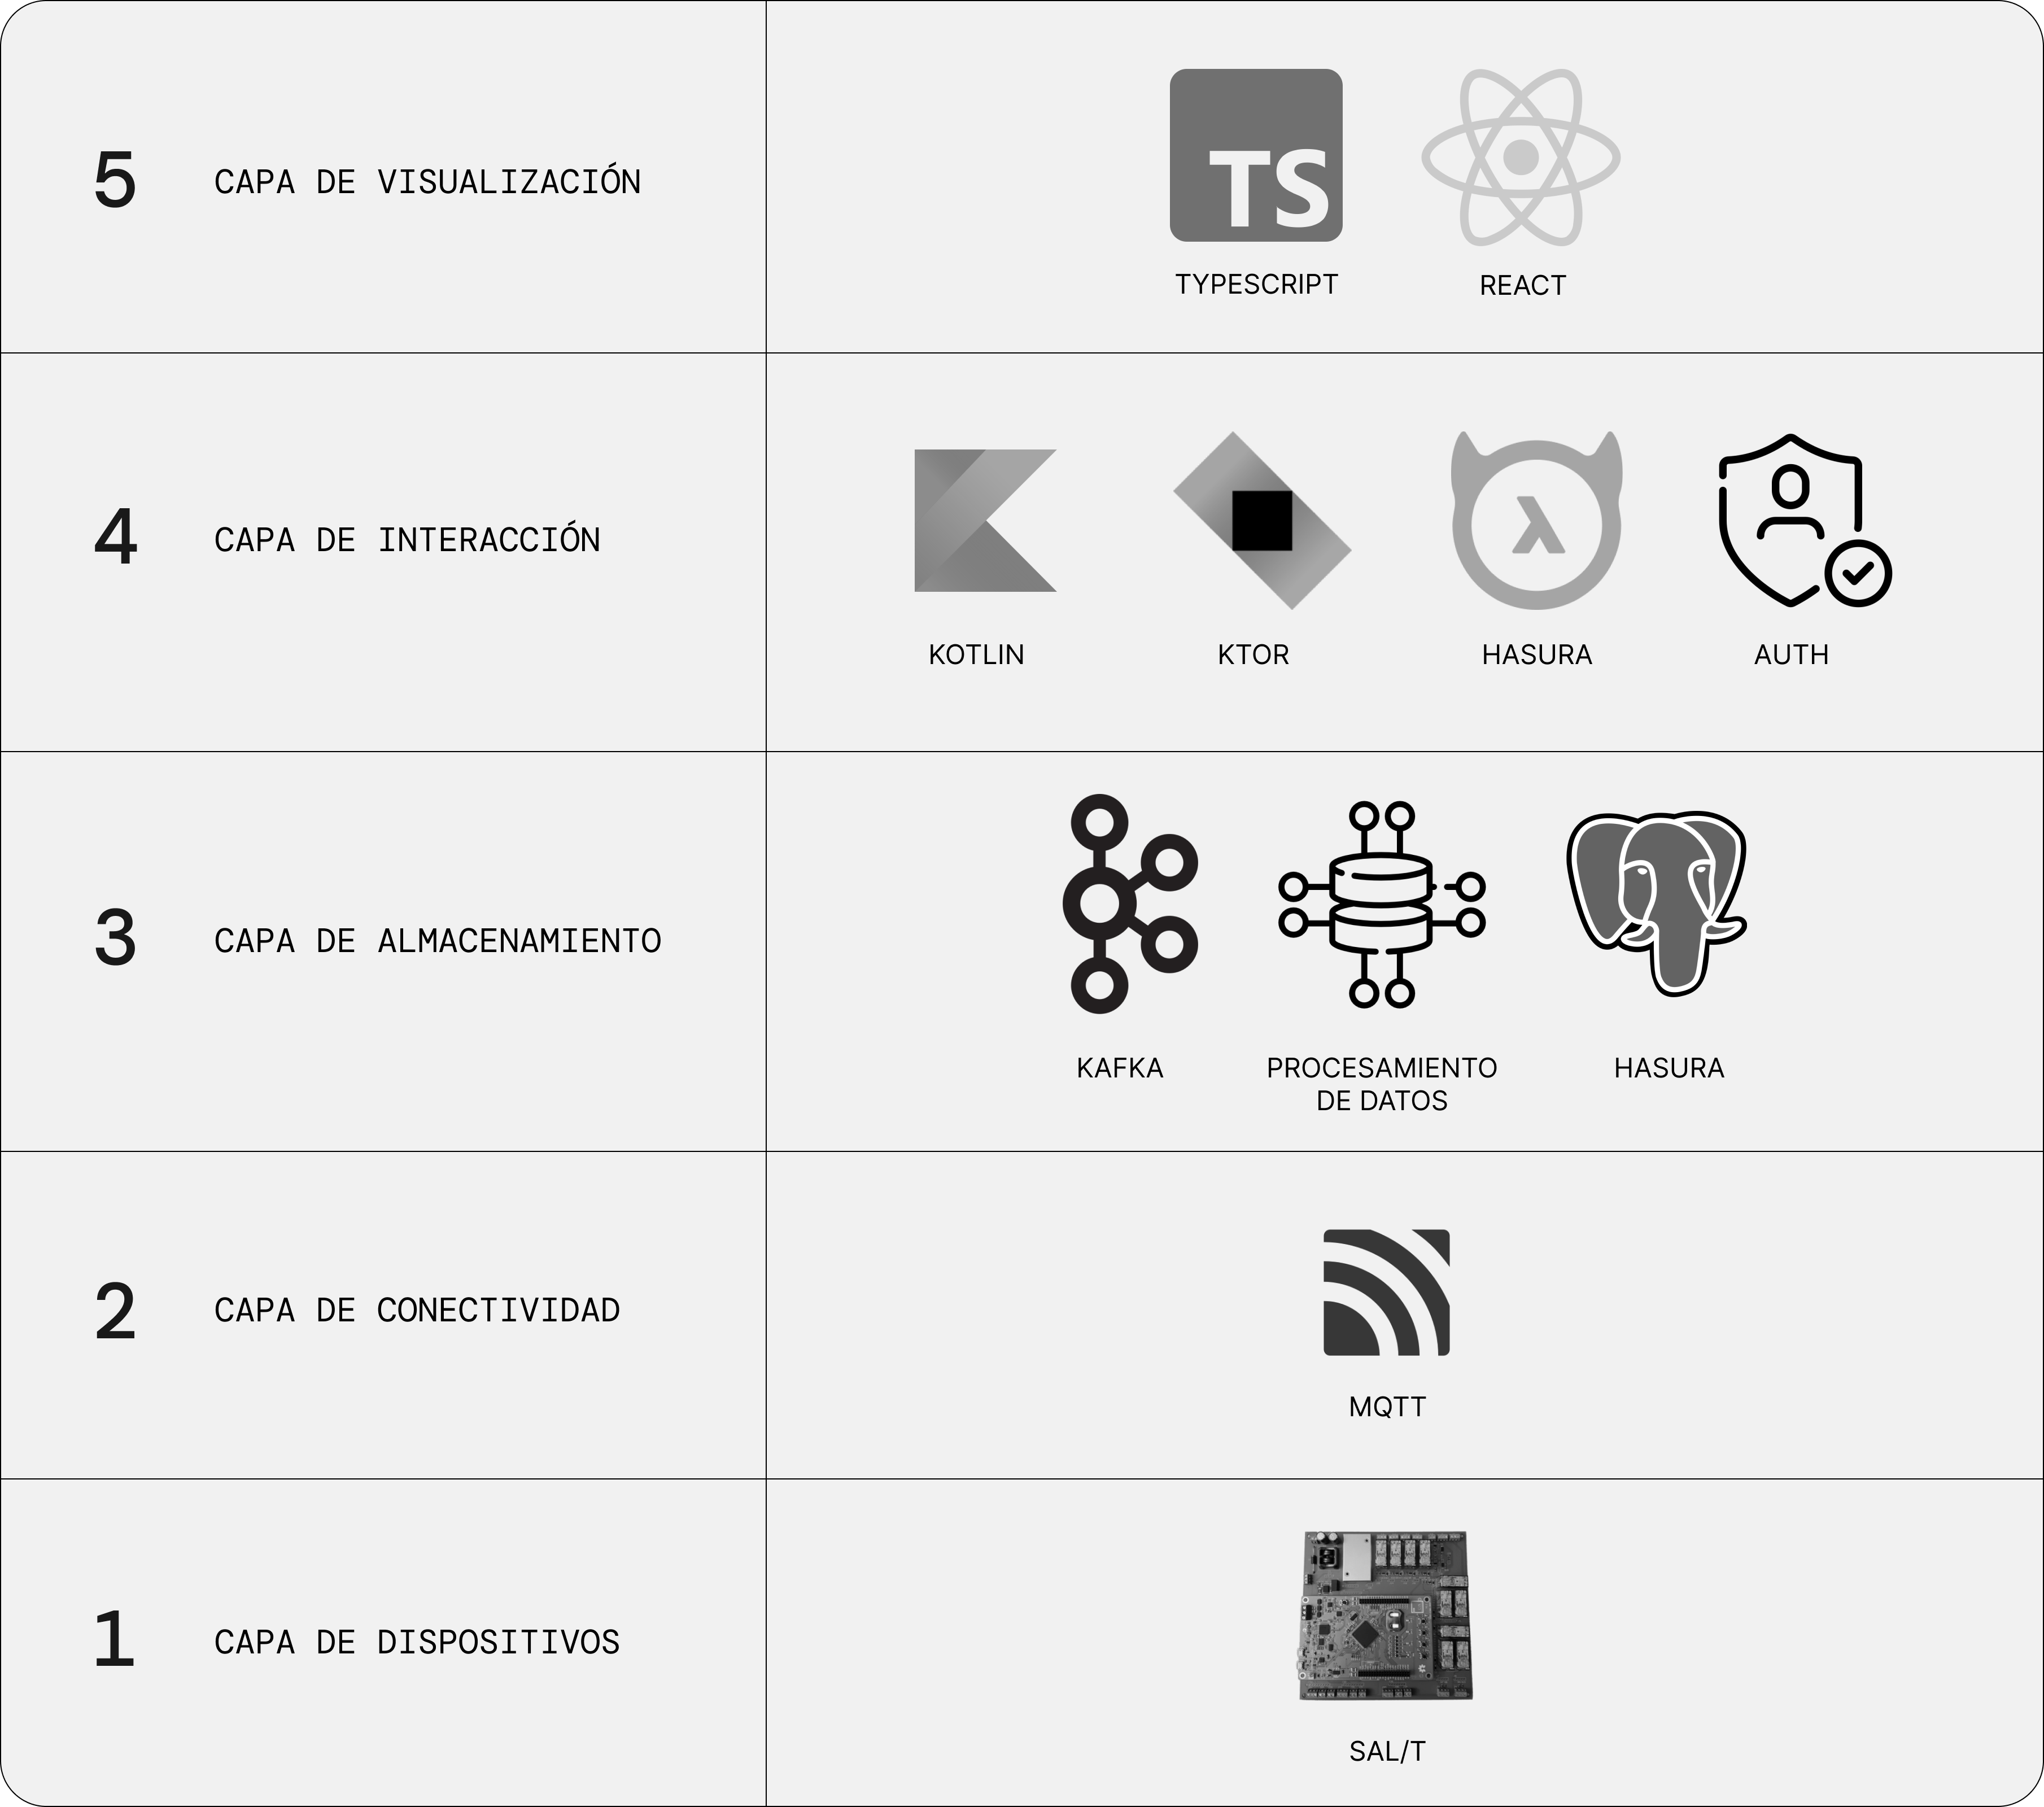
\includegraphics[width=.48\textwidth]{images/iot-stack-v2.1.png}
\caption{Arquitectura de la Central Operativa SAL/T.}
\label{fig:diagBloques}
\end{figure}

\subsection{Capa de dispositivos}

Sobre la base de un prototipo del Sistema de Aislamiento Limitado o Total, \textit{SAL/T}, se desarolló, en el kit de desarrollo \textit{Nucleo F429} \cite{b8}, un cliente \textit{MQTT} que permite la publicación de la velocidad de la formación y de los parámetros provistos por los subsistemas de falla, entre otras variables; y llegado el caso, el dispositivo pueda realizar la lectura de diferentes parámetros configurables.

\subsection{Capa de conectividad}

Para la comunicación entre los dispositivos \textit{SAL/T} y la capa de almacenamiento se utiliza un \textit{Broker MQTT} que oficia de orquestador entre el cliente, el dispositivo \textit{SAL/T} que publica los mensajes y \textit{Apache Kafka} \cite{b9}, un sistema distribuido que realiza la lectura de la información y su posterior procesamiento. 

Dado que los mensajes intercambiados entre las partes contienen información sensible, se ha optado por agregar la capa de seguridad \textit{TLS} \cite{b10}. En este sentido, resulta indispensable utilizar el certificado \textit{X509} \cite{b11} para prevenir ataques del tipo \textit{adversary-in-the-middle} \cite{b12} y utilizar certificados emitidos por autoridades reconocidas.


\subsection{Capa de almacenamiento}

La capa de almacenamiento se encuentra constituida por el sistema distribuido \textit{Kafka} que se encarga de almacenar los datos de la aplicación. Entre ellos se destacan los mensajes MQTT enviados por los dispositivos SAL/T, como también la información referida a las formaciones y a los SAL/T que las ocupan. Además, se tienen servicios de procesamiento de datos que se encargan de adaptar la información de los tópicos en datos que posteriormente serán consumidos por los servicios que integran la capa superior.

Por otro lado, se tiene una base de datos relacional \textit{PostgreSQL} \cite{b13} que se utiliza para almacenar los datos del servicio de autenticación y el motor que facilita la interacción con la plataforma web. Los conectores se encargan de insertar los datos que se quieran disponer a la capa de visualización.

\begin{figure}[ht]
\centering 
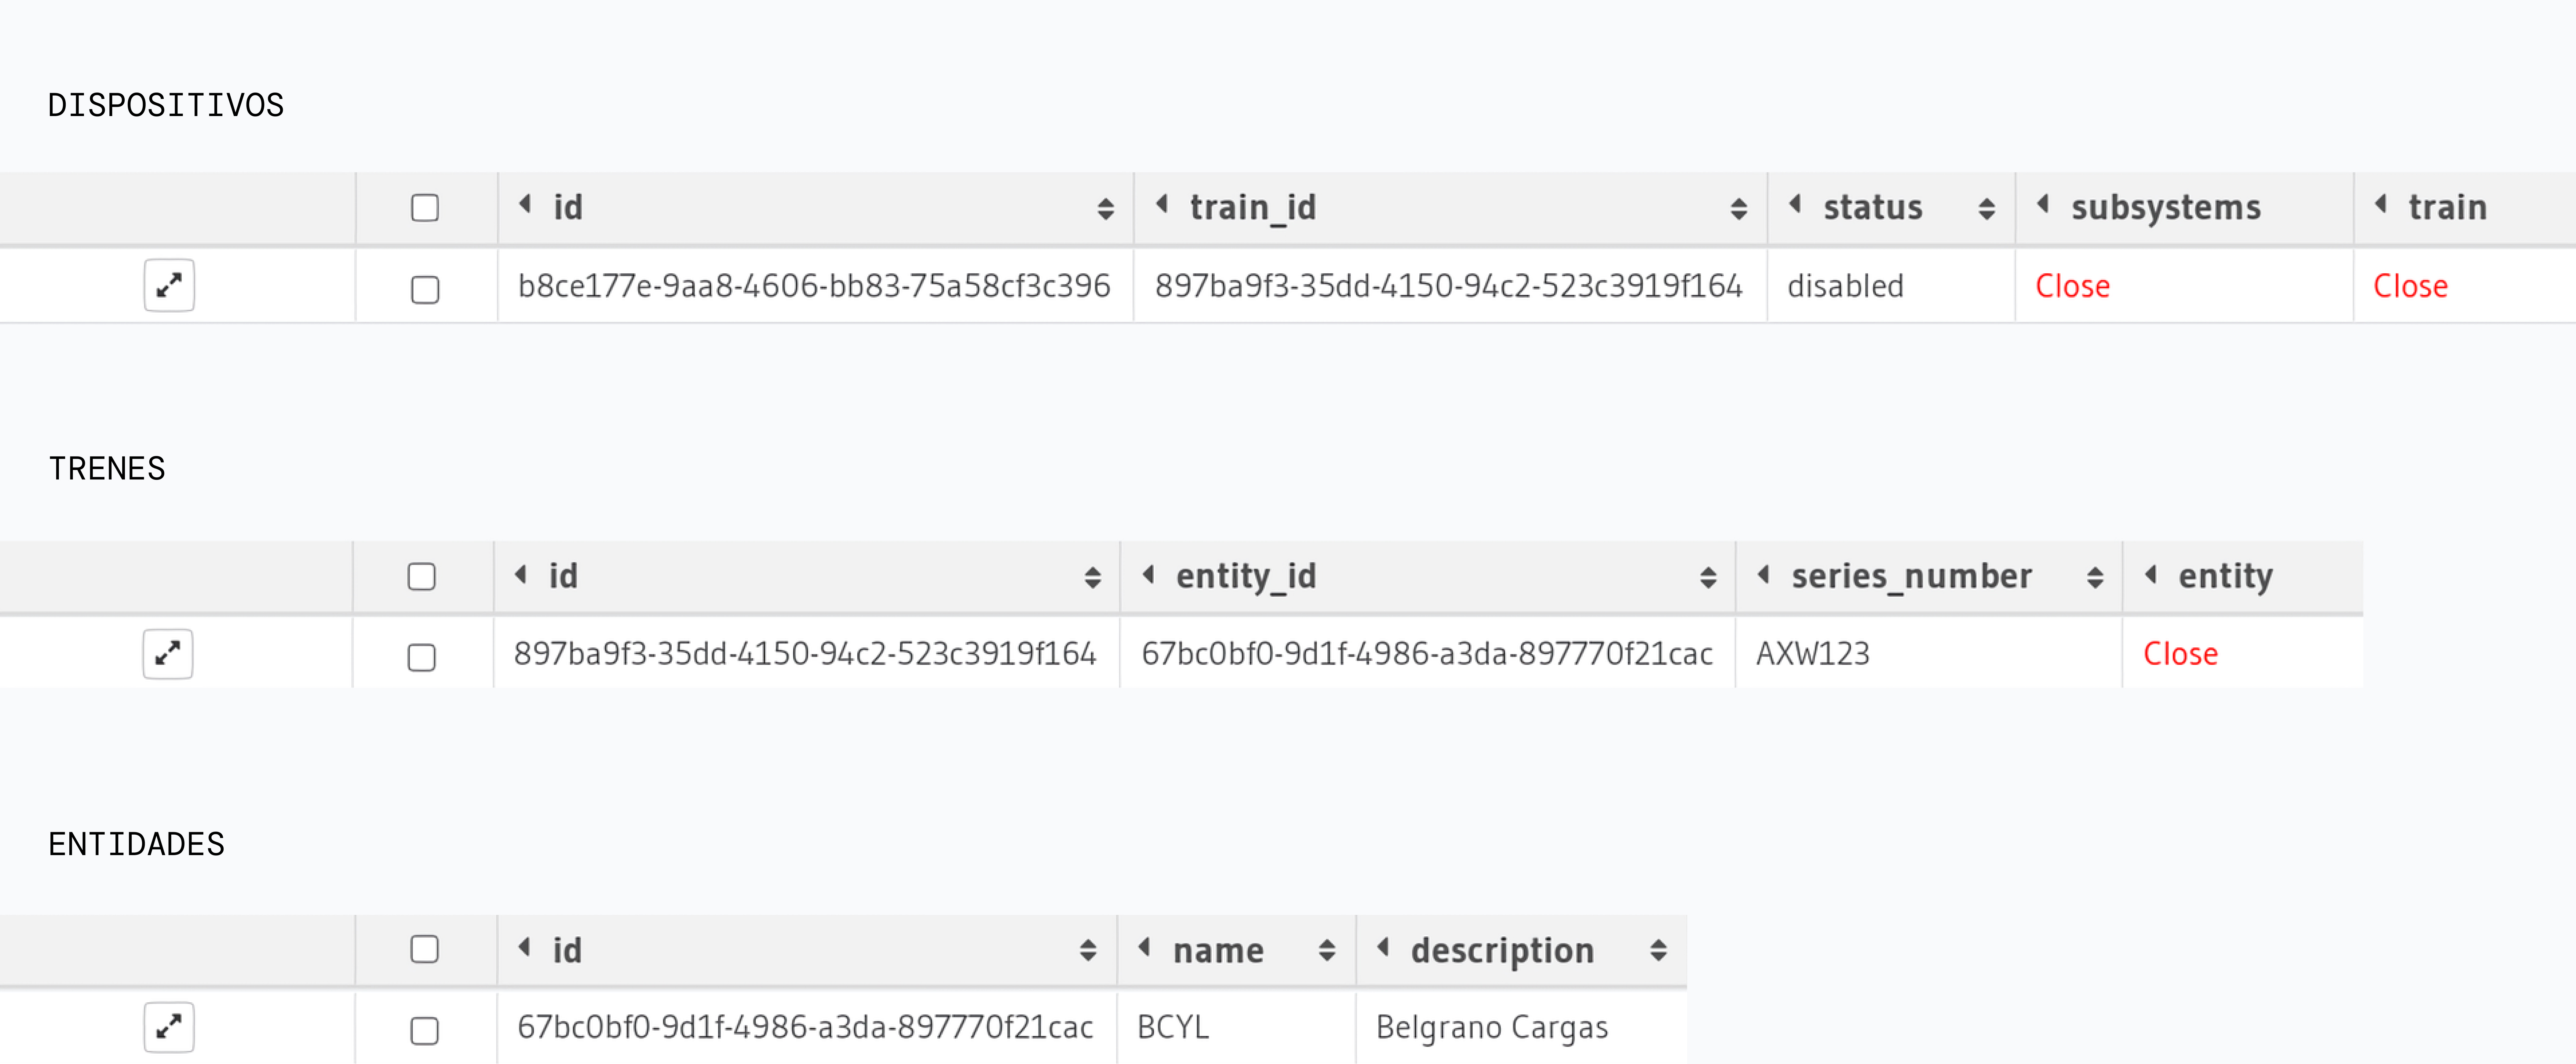
\includegraphics[width=.5\textwidth]{images/salt_table_v2.1.jpg}
\caption{Modelo de datos de los dispositivos, trenes y entidades.}
\label{fig:devicesTrainEntity}
\end{figure}

\begin{figure}[ht]
\centering 
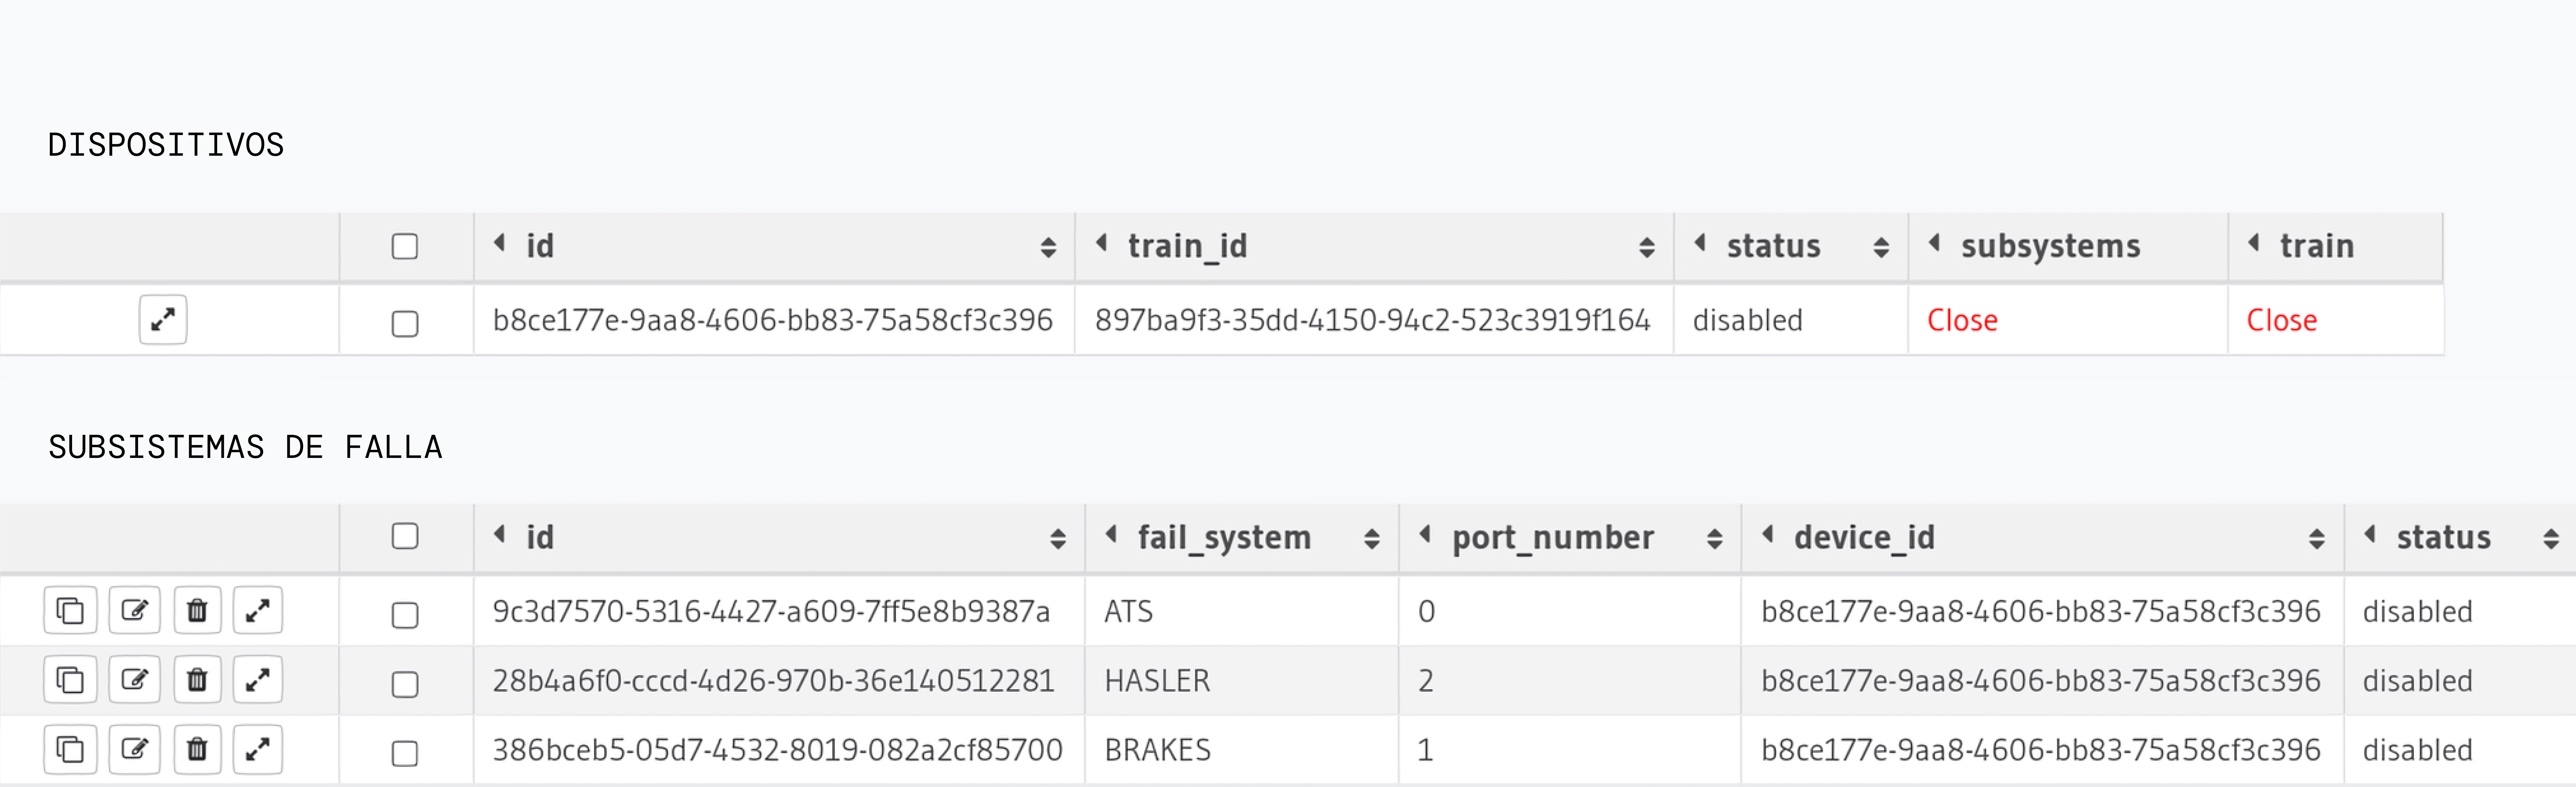
\includegraphics[width=.5\textwidth]{images/fail_system_v2.1.jpg}
\caption{Modelo de datos de los dispositivos y sus subsistemas de fallas.}
\label{fig:devicesSubsystems}
\end{figure}

En la figura \ref{fig:devicesTrainEntity} se observa el modelo de datos que representa a los dispositivos SAL/T, las formaciones y las entidades. 
El primero cuenta con un identificador del dispositivo en el sistema, el estado de operación y una referencia al tren en el que se desplegó el artefacto. 
El modelo de la formación está enriquecido con la entidad a la que pertenece y el numero de serie del tren. 
Por último, las entidades están compuestas por nombre y descripción.
Luego, en la imagen \ref{fig:devicesSubsystems} se aprecian los subsistemas de fallas relacionados con el dispositivo SAL/T.
Su modelo esta integrado con el nombre del subsistema, el id del dispositivo al que está asociado y el estado actual del mismo. 

\subsection{Capa de interacción}

La capa de interacción se encuentra conformada por tres unidades. Por un lado, se ha desarrollado en el lenguaje \textit{Kotlin} \cite{b14} en conjunto con el \textit{framework} \textit{Ktor} \cite{b15}, un microservicio de autenticación donde es posible la gestión de los usuarios con sus respectivos roles y también el \textit{backend}. Entre sus tareas principales se encuentran las relacionadas al protocolo \textit{MQTT} para la actualización de los certificados que brindan seguridad a las comunicaciones, mediante el uso de la capa de seguridad \textit{TLS}, y la indexación de los eventos que se publiquen en tiempo real; como la configuración general que permite el funcionamiento integral de los servicios y módulos dispuestos en el sistema. \\

Además, se dispone del motor \textit{Hasura} \cite{b16}, el cual se encuentra conectado a una base de datos relacional (\textit{PostgreSQL}) basado en el lenguaje de consulta estructurado \textit{SQL} \cite{b17}, que permite exponer una \textit{API GraphQL} \cite{b18} a aquellos clientes que deseen obtener una visualización del modelo de datos propuesto en que se conjuga la información de cada formación ferroviaria con su correspondiente dispositivo \textit{SAL/T} y diseño destinado al \textit{frontend}. Más aún, el enlace permite realizar modificaciones y hasta remociones de las columnas propuestas en las tablas de cada esquema dentro de la base de datos.


\subsection{Capa de visualización}

En esta capa, se ha utilizado el lenguaje de programación \textit{TypeScript} \cite{b19} junto con la biblioteca gráfica \textit{React} \cite{b20} para brindar una web reactiva en la que se elaboraron los formularios, las tablas y los paneles a partir de la explotación en de los datos almacenados en la base de datos. Cabe destacar que la plataforma web se encuentra condicionada por el rol y la entidad ferroviaria a la que pertenece cada usuario.

En la figura \ref{fig:dashboard} se puede apreciar el dashboard de la central operativa al que tendrán acceso los operadores de cada entidad.
En el mismo se observan distintas tarjetas con el estado de cada subsistema de fallas y del tren, como así también un velocímetro que
informa la velocidad de la formación.

\begin{figure}[ht]
\centering 
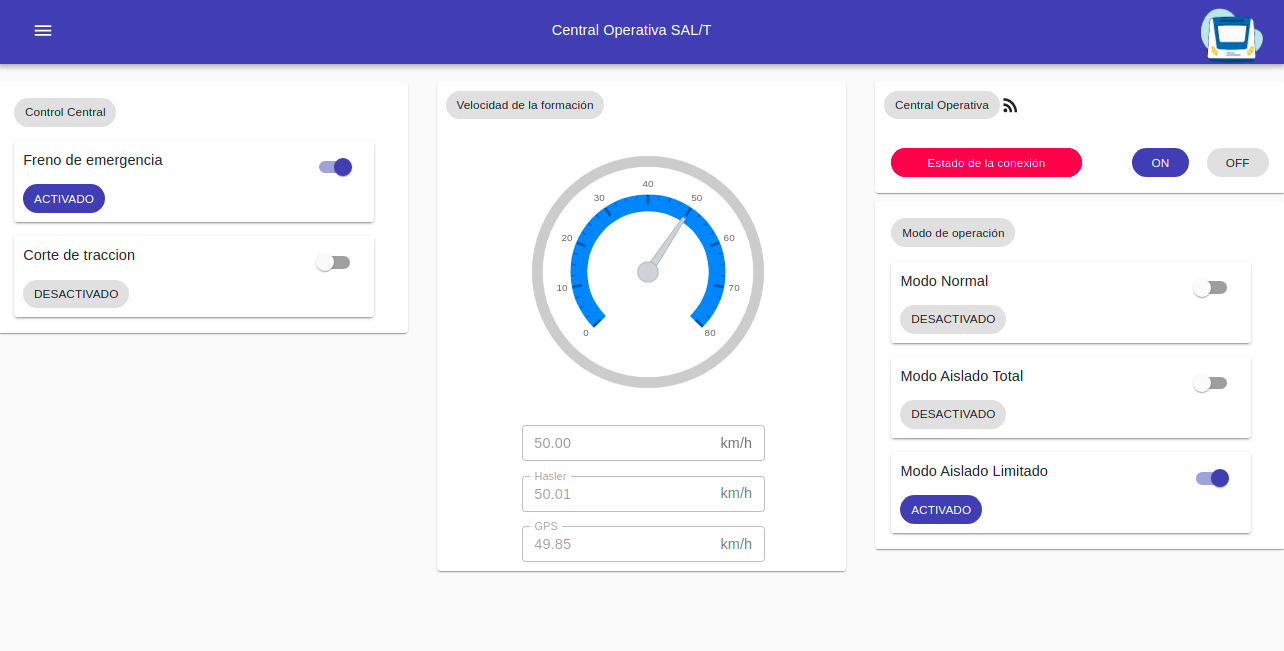
\includegraphics[width=.47\textwidth]{images/cental.png}
\caption{Panel de control de la central operativa.}
\label{fig:dashboard}
\end{figure}
